\documentclass[12pt,a4paper]{article}
\usepackage{geometry}
\usepackage{graphicx}
\usepackage{amsmath}
\usepackage{amssymb}
\usepackage{array}
\usepackage{hyperref}
\usepackage{float}
\usepackage{tikz}
\usepackage{circuitikz}
\usetikzlibrary{shapes}
\usetikzlibrary{shapes, arrows.meta, positioning}
\usepackage{caption}
\usepackage{subcaption}

\geometry{margin=1in}

\begin{document}

\begin{titlepage}
    \centering
    \begin{center}
        
\includegraphics[width=0.5\textwidth]{logo.png}
    \end{center}
\begin{center}
    \textbf{Department of Computer Science and Engineering}\\
    Premier University
\end{center}
\begin{center}
    \textnormal{EEE 310 : Communication Engineering Laboratory}
\end{center}
    \huge
    \textbf{Project Proposal Report}\\
    \vspace{0.5in}
    \LARGE
    \textbf{Amplitude Shift Keying (ASK)}\\
    \vspace{1in}
    \large
    \textbf {Submitted by}\\
    \begin{center}
        \renewcommand{\arraystretch}{1.5} % Adjusts vertical spacing in the table
        \begin{tabular}{|>{\raggedright\arraybackslash}p{0.6\textwidth}|p{0.3\textwidth}|} % Adjust column widths
        \hline
        \textbf{Name} & \textbf{ID} \\
        \hline
        Mohammad Hafizur Rahman Sakib & 0222210005101118 \\
        \hline
        Arnab Shikder & 0222210005101098 \\
        \hline
        Shuvra Roy & 0222210005101093 \\
        \hline
        Sayed Hossain & 0222210005101102 \\
        \hline
        Mohammad Asmual Hoque Yousha & 0222210005101121 \\
        \hline
        Mohammad Ohidul Alam & 0222210005101123 \\
        \hline
        \end{tabular}
        \end{center}
    \vspace{0.5in}
 
    \begin{minipage}[t]{0.5\textwidth}
        \textbf{Submitted to:}
        \\ Sharith Dhar
        \\Lecturer,Department of EEE\\ Premier University, Chittagong
    \end{minipage}%
    \begin{minipage}[t]{0.6\textwidth}
        \raggedleft
        \textbf{Remarks}\\
        \vspace{0.5cm} % Adjust vertical space for remarks
        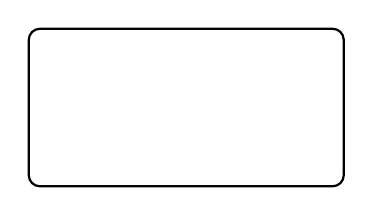
\begin{tikzpicture}
            \draw[thick, rounded corners] (0,0) rectangle (4,2);
        \end{tikzpicture}
    \end{minipage}

    \date{\today}
    \vfill
\end{titlepage}

\newpage

\section*{Introduction :}
Amplitude Shift Keying (ASK) is a digital modulation technique where the amplitude of a carrier signal is varied according to the binary data being transmitted. This project focuses on the design and implementation of the ASK modulation process to explore its efficiency and applications in digital communication systems.

\section*{Objectives :}
The main objectives of this project are to:
\begin{itemize}
    \item Understand the principles of ASK modulation.
    \item Design and develop an ASK modulator.
    \item Simulate and analyze the performance of the ASK modulator.
    \item Evaluate the efficiency of ASK modulation in various scenarios.
\end{itemize}


% Block Diagram
\section*{Block Diagram :}

\begin{figure}[htbp]
    \centering
    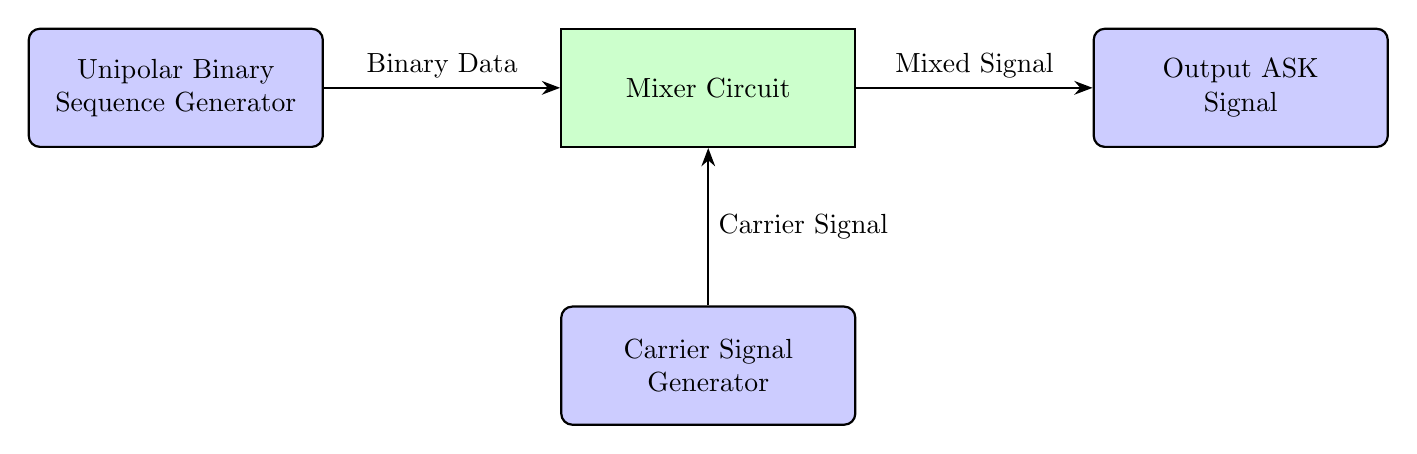
\begin{tikzpicture}[node distance=2cm and 3cm, auto, thick,
        block/.style={draw, fill=blue!20, text width=3.5cm, minimum height=1.5cm, align=center, rounded corners},
        ellipse/.style={draw, fill=green!20, text width=3.5cm, minimum height=1.5cm, align=center},
        arrow/.style={-Stealth, thick},
        every node/.style={align=center}]

        % Nodes
        \node [block] (binary) {Unipolar Binary\\Sequence Generator};
        \node [ellipse, right=of binary] (mixer) {Mixer Circuit};
        \node [block, below=of mixer] (carrier) {Carrier Signal\\Generator};
        \node [block, right=of mixer] (output) {Output ASK\\Signal};

        % Arrows
        \draw [arrow] (binary) -- node[above] {Binary Data} (mixer);
        \draw [arrow] (mixer) -- node[above] {Mixed Signal} (output);
        \draw [arrow] (carrier) -- node[right] {Carrier Signal} (mixer);
\end{tikzpicture}
    \caption{Block Diagram of ASK Modulation}
    \label{fig:ask_block_diagram}
\end{figure}



\section*{ASK Modulation Waveforms :}
\begin{center}
    \includegraphics[width=1.0\textwidth]{waves.png}
    \newline
    \textbf {Fig 02 : ASK Modulation Waveforms}
\end{center}


\section*{Circuit Diagram :}
\begin{center}
    \includegraphics[width=1.0\textwidth]{circuit_diagram.png}
    \newline
    \textbf {Fig 03 : ASK Modulation Circuit}
\end{center}



\section*{Conclusion :}

In conclusion, this project successfully designed and simulated an ASK modulator, providing valuable insights into its practical applications and performance characteristics in digital communication. ASK modulation's versatility and effectiveness in transmitting binary data through amplitude variation were clearly demonstrated. Its straightforward implementation and robust performance across different conditions highlight its enduring relevance in modern telecommunications.

\end{document}
